% Options for packages loaded elsewhere
\PassOptionsToPackage{unicode}{hyperref}
\PassOptionsToPackage{hyphens}{url}
\PassOptionsToPackage{dvipsnames,svgnames,x11names}{xcolor}
%
\documentclass[
  letterpaper,
  DIV=11,
  numbers=noendperiod]{scrartcl}

\usepackage{amsmath,amssymb}
\usepackage{iftex}
\ifPDFTeX
  \usepackage[T1]{fontenc}
  \usepackage[utf8]{inputenc}
  \usepackage{textcomp} % provide euro and other symbols
\else % if luatex or xetex
  \usepackage{unicode-math}
  \defaultfontfeatures{Scale=MatchLowercase}
  \defaultfontfeatures[\rmfamily]{Ligatures=TeX,Scale=1}
\fi
\usepackage{lmodern}
\ifPDFTeX\else  
    % xetex/luatex font selection
\fi
% Use upquote if available, for straight quotes in verbatim environments
\IfFileExists{upquote.sty}{\usepackage{upquote}}{}
\IfFileExists{microtype.sty}{% use microtype if available
  \usepackage[]{microtype}
  \UseMicrotypeSet[protrusion]{basicmath} % disable protrusion for tt fonts
}{}
\makeatletter
\@ifundefined{KOMAClassName}{% if non-KOMA class
  \IfFileExists{parskip.sty}{%
    \usepackage{parskip}
  }{% else
    \setlength{\parindent}{0pt}
    \setlength{\parskip}{6pt plus 2pt minus 1pt}}
}{% if KOMA class
  \KOMAoptions{parskip=half}}
\makeatother
\usepackage{xcolor}
\setlength{\emergencystretch}{3em} % prevent overfull lines
\setcounter{secnumdepth}{-\maxdimen} % remove section numbering
% Make \paragraph and \subparagraph free-standing
\makeatletter
\ifx\paragraph\undefined\else
  \let\oldparagraph\paragraph
  \renewcommand{\paragraph}{
    \@ifstar
      \xxxParagraphStar
      \xxxParagraphNoStar
  }
  \newcommand{\xxxParagraphStar}[1]{\oldparagraph*{#1}\mbox{}}
  \newcommand{\xxxParagraphNoStar}[1]{\oldparagraph{#1}\mbox{}}
\fi
\ifx\subparagraph\undefined\else
  \let\oldsubparagraph\subparagraph
  \renewcommand{\subparagraph}{
    \@ifstar
      \xxxSubParagraphStar
      \xxxSubParagraphNoStar
  }
  \newcommand{\xxxSubParagraphStar}[1]{\oldsubparagraph*{#1}\mbox{}}
  \newcommand{\xxxSubParagraphNoStar}[1]{\oldsubparagraph{#1}\mbox{}}
\fi
\makeatother

\usepackage{color}
\usepackage{fancyvrb}
\newcommand{\VerbBar}{|}
\newcommand{\VERB}{\Verb[commandchars=\\\{\}]}
\DefineVerbatimEnvironment{Highlighting}{Verbatim}{commandchars=\\\{\}}
% Add ',fontsize=\small' for more characters per line
\usepackage{framed}
\definecolor{shadecolor}{RGB}{241,243,245}
\newenvironment{Shaded}{\begin{snugshade}}{\end{snugshade}}
\newcommand{\AlertTok}[1]{\textcolor[rgb]{0.68,0.00,0.00}{#1}}
\newcommand{\AnnotationTok}[1]{\textcolor[rgb]{0.37,0.37,0.37}{#1}}
\newcommand{\AttributeTok}[1]{\textcolor[rgb]{0.40,0.45,0.13}{#1}}
\newcommand{\BaseNTok}[1]{\textcolor[rgb]{0.68,0.00,0.00}{#1}}
\newcommand{\BuiltInTok}[1]{\textcolor[rgb]{0.00,0.23,0.31}{#1}}
\newcommand{\CharTok}[1]{\textcolor[rgb]{0.13,0.47,0.30}{#1}}
\newcommand{\CommentTok}[1]{\textcolor[rgb]{0.37,0.37,0.37}{#1}}
\newcommand{\CommentVarTok}[1]{\textcolor[rgb]{0.37,0.37,0.37}{\textit{#1}}}
\newcommand{\ConstantTok}[1]{\textcolor[rgb]{0.56,0.35,0.01}{#1}}
\newcommand{\ControlFlowTok}[1]{\textcolor[rgb]{0.00,0.23,0.31}{\textbf{#1}}}
\newcommand{\DataTypeTok}[1]{\textcolor[rgb]{0.68,0.00,0.00}{#1}}
\newcommand{\DecValTok}[1]{\textcolor[rgb]{0.68,0.00,0.00}{#1}}
\newcommand{\DocumentationTok}[1]{\textcolor[rgb]{0.37,0.37,0.37}{\textit{#1}}}
\newcommand{\ErrorTok}[1]{\textcolor[rgb]{0.68,0.00,0.00}{#1}}
\newcommand{\ExtensionTok}[1]{\textcolor[rgb]{0.00,0.23,0.31}{#1}}
\newcommand{\FloatTok}[1]{\textcolor[rgb]{0.68,0.00,0.00}{#1}}
\newcommand{\FunctionTok}[1]{\textcolor[rgb]{0.28,0.35,0.67}{#1}}
\newcommand{\ImportTok}[1]{\textcolor[rgb]{0.00,0.46,0.62}{#1}}
\newcommand{\InformationTok}[1]{\textcolor[rgb]{0.37,0.37,0.37}{#1}}
\newcommand{\KeywordTok}[1]{\textcolor[rgb]{0.00,0.23,0.31}{\textbf{#1}}}
\newcommand{\NormalTok}[1]{\textcolor[rgb]{0.00,0.23,0.31}{#1}}
\newcommand{\OperatorTok}[1]{\textcolor[rgb]{0.37,0.37,0.37}{#1}}
\newcommand{\OtherTok}[1]{\textcolor[rgb]{0.00,0.23,0.31}{#1}}
\newcommand{\PreprocessorTok}[1]{\textcolor[rgb]{0.68,0.00,0.00}{#1}}
\newcommand{\RegionMarkerTok}[1]{\textcolor[rgb]{0.00,0.23,0.31}{#1}}
\newcommand{\SpecialCharTok}[1]{\textcolor[rgb]{0.37,0.37,0.37}{#1}}
\newcommand{\SpecialStringTok}[1]{\textcolor[rgb]{0.13,0.47,0.30}{#1}}
\newcommand{\StringTok}[1]{\textcolor[rgb]{0.13,0.47,0.30}{#1}}
\newcommand{\VariableTok}[1]{\textcolor[rgb]{0.07,0.07,0.07}{#1}}
\newcommand{\VerbatimStringTok}[1]{\textcolor[rgb]{0.13,0.47,0.30}{#1}}
\newcommand{\WarningTok}[1]{\textcolor[rgb]{0.37,0.37,0.37}{\textit{#1}}}

\providecommand{\tightlist}{%
  \setlength{\itemsep}{0pt}\setlength{\parskip}{0pt}}\usepackage{longtable,booktabs,array}
\usepackage{calc} % for calculating minipage widths
% Correct order of tables after \paragraph or \subparagraph
\usepackage{etoolbox}
\makeatletter
\patchcmd\longtable{\par}{\if@noskipsec\mbox{}\fi\par}{}{}
\makeatother
% Allow footnotes in longtable head/foot
\IfFileExists{footnotehyper.sty}{\usepackage{footnotehyper}}{\usepackage{footnote}}
\makesavenoteenv{longtable}
\usepackage{graphicx}
\makeatletter
\newsavebox\pandoc@box
\newcommand*\pandocbounded[1]{% scales image to fit in text height/width
  \sbox\pandoc@box{#1}%
  \Gscale@div\@tempa{\textheight}{\dimexpr\ht\pandoc@box+\dp\pandoc@box\relax}%
  \Gscale@div\@tempb{\linewidth}{\wd\pandoc@box}%
  \ifdim\@tempb\p@<\@tempa\p@\let\@tempa\@tempb\fi% select the smaller of both
  \ifdim\@tempa\p@<\p@\scalebox{\@tempa}{\usebox\pandoc@box}%
  \else\usebox{\pandoc@box}%
  \fi%
}
% Set default figure placement to htbp
\def\fps@figure{htbp}
\makeatother

\KOMAoption{captions}{tableheading}
\makeatletter
\@ifpackageloaded{caption}{}{\usepackage{caption}}
\AtBeginDocument{%
\ifdefined\contentsname
  \renewcommand*\contentsname{Tabla de contenidos}
\else
  \newcommand\contentsname{Tabla de contenidos}
\fi
\ifdefined\listfigurename
  \renewcommand*\listfigurename{Listado de Figuras}
\else
  \newcommand\listfigurename{Listado de Figuras}
\fi
\ifdefined\listtablename
  \renewcommand*\listtablename{Listado de Tablas}
\else
  \newcommand\listtablename{Listado de Tablas}
\fi
\ifdefined\figurename
  \renewcommand*\figurename{Figura}
\else
  \newcommand\figurename{Figura}
\fi
\ifdefined\tablename
  \renewcommand*\tablename{Tabla}
\else
  \newcommand\tablename{Tabla}
\fi
}
\@ifpackageloaded{float}{}{\usepackage{float}}
\floatstyle{ruled}
\@ifundefined{c@chapter}{\newfloat{codelisting}{h}{lop}}{\newfloat{codelisting}{h}{lop}[chapter]}
\floatname{codelisting}{Listado}
\newcommand*\listoflistings{\listof{codelisting}{Listado de Listados}}
\makeatother
\makeatletter
\makeatother
\makeatletter
\@ifpackageloaded{caption}{}{\usepackage{caption}}
\@ifpackageloaded{subcaption}{}{\usepackage{subcaption}}
\makeatother

\ifLuaTeX
\usepackage[bidi=basic]{babel}
\else
\usepackage[bidi=default]{babel}
\fi
\babelprovide[main,import]{spanish}
% get rid of language-specific shorthands (see #6817):
\let\LanguageShortHands\languageshorthands
\def\languageshorthands#1{}
\usepackage{bookmark}

\IfFileExists{xurl.sty}{\usepackage{xurl}}{} % add URL line breaks if available
\urlstyle{same} % disable monospaced font for URLs
\hypersetup{
  pdftitle={Taller RML (Parte 1) - Gr4},
  pdfauthor={Luis David Hernandez; Daniel Felipe villa Rengifo; Juan Gabriel Carvajal},
  pdflang={es},
  colorlinks=true,
  linkcolor={blue},
  filecolor={Maroon},
  citecolor={Blue},
  urlcolor={Blue},
  pdfcreator={LaTeX via pandoc}}


\title{Taller RML (Parte 1) - Gr4}
\usepackage{etoolbox}
\makeatletter
\providecommand{\subtitle}[1]{% add subtitle to \maketitle
  \apptocmd{\@title}{\par {\large #1 \par}}{}{}
}
\makeatother
\subtitle{Departamento de Estadística - UNALMED}
\author{Luis David Hernandez \and Daniel Felipe villa Rengifo \and Juan
Gabriel Carvajal}
\date{}

\begin{document}
\maketitle


\begin{enumerate}
\def\labelenumi{\arabic{enumi}.}
\tightlist
\item
  Realice una descripción de la base de datos. Contextualice el problema
  y explique cada una de las variables involucradas en el modelo.
  (https://www.codersarts.com/post/predict-boston-house-prices-using-python-linear-regression).
\end{enumerate}

\section{Descripción de la base de
datos}\label{descripciuxf3n-de-la-base-de-datos}

Tomaremos el conjunto de datos de Vivienda que contiene información
sobre diferentes casas en Boston. Hay 506 muestras y 13 variables de
características en este conjunto de datos. El objetivo es predecir el
valor de los precios de la casa utilizando las características dadas.

La descripción de todas las características se proporciona a
continuación:

\begin{itemize}
\item
  \textbf{CRIM}: tasa de criminalidad per cápita por ciudad
\item
  \textbf{ZN}: proporción de terrenos residenciales zonificados para
  lotes de más de 25 000 pies cuadrados
\item
  \textbf{INDUS:} proporción de acres de negocios no minoristas por
  ciudad
\item
  \textbf{CHAS}: variable ficticia de Charles River (= 1 si el terreno
  limita con el río; 0 en caso contrario) NOX: concentración de óxido
  nítrico (partes por 10 millones)
\item
  \textbf{RM}: número promedio de habitaciones por vivienda
\item
  \textbf{AGE}: proporción de unidades ocupadas por sus propietarios
  construidas antes de 1940 DIS: distancias ponderadas a cinco centros
  de empleo de Boston
\item
  \textbf{RAD}: índice de accesibilidad a carreteras radiales
\item
  \textbf{TAX}: tasa de impuesto a la propiedad de valor total por cada
  \$10 000
\item
  \textbf{PTRATIO}: proporción de alumnos por maestro por ciudad B:
  1000(Bk --- 0,63)², donde Bk es la proporción de {[}personas de
  afroamericanas {[}descendencia{]} por ciudad
\item
  \textbf{LSTAT}: Porcentaje de la población de estatus inferior
\item
  \textbf{MEDV}: Valor medio de las viviendas ocupadas por sus
  propietarios en miles de dólares
\end{itemize}

Los precios de las viviendas indicados por la variable \textbf{MEDV} son
nuestra variable objetivo y las restantes son las variables
características en función de las cuales predeciremos el valor de una
vivienda.

\begin{enumerate}
\def\labelenumi{\arabic{enumi}.}
\setcounter{enumi}{1}
\tightlist
\item
  Realice un análisis descriptivo de las variables que se van a tener en
  cuenta en el modelo. Concluya.
\end{enumerate}

\pandocbounded{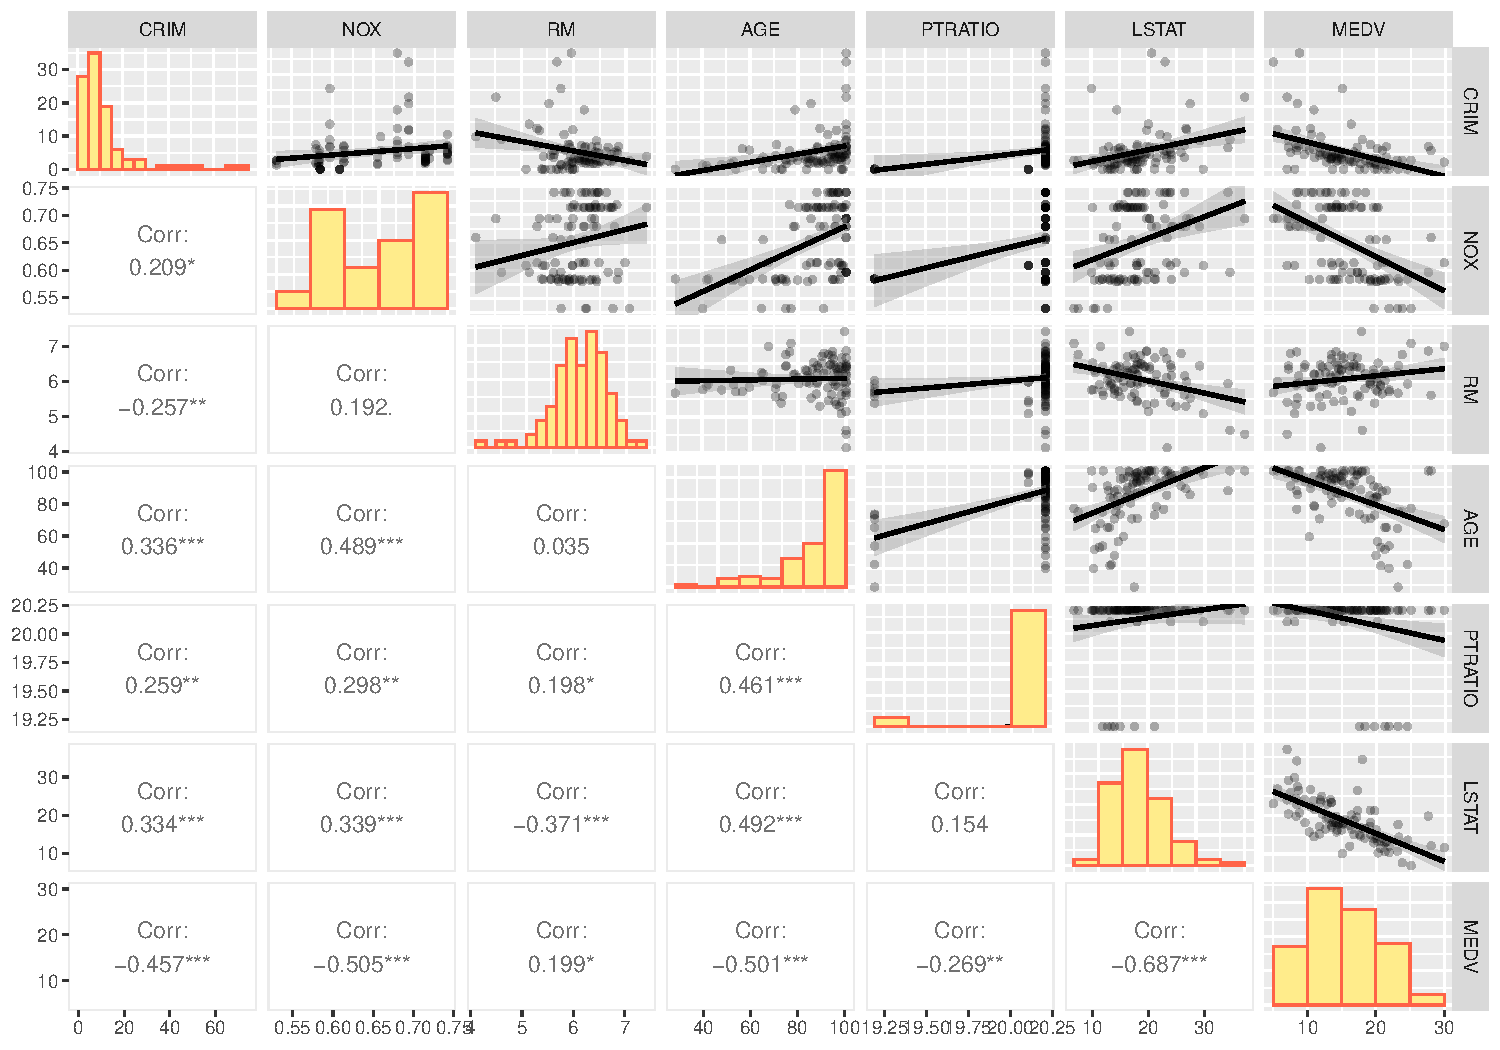
\includegraphics[keepaspectratio]{Taller_4_files/figure-pdf/unnamed-chunk-2-1.pdf}}

\textbf{Correlaciones}: MEDV tiene una fuerte correlación positiva con
RM (número promedio de habitaciones por vivienda), lo que indica que las
viviendas con más habitaciones tienden a tener un valor más alto. Por
otro lado, MEDV tiene una fuerte correlación negativa con LSTAT
(porcentaje de la población de estatus inferior), lo que sugiere que las
viviendas en áreas con mayor porcentaje de población de bajos ingresos
tienden a tener un valor más bajo.

\textbf{Otras variables}: CRIM (tasa de criminalidad): Tiene una
correlación negativa moderada con MEDV, lo que indica que las viviendas
en áreas con mayor criminalidad tienden a tener un valor más bajo.RM
(número de habitaciones): Además de su fuerte correlación con MEDV, RM
también muestra una correlación positiva con AGE (proporción de unidades
ocupadas por sus propietarios construidas antes de 1940). Esto podría
indicar que las viviendas más antiguas tienden a tener más
habitaciones.LSTAT (porcentaje de población de bajos ingresos): Además
de su correlación negativa con MEDV, LSTAT también muestra correlaciones
negativas con RM y una correlación positiva con CRIM. Esto sugiere que
las áreas con mayor porcentaje de población de bajos ingresos tienden a
tener viviendas más pequeñas y mayor criminalidad.

\section{Prueba de normalidad}\label{prueba-de-normalidad}

\begin{Shaded}
\begin{Highlighting}[]
\FunctionTok{shapiro.test}\NormalTok{(datos4}\SpecialCharTok{$}\NormalTok{MEDV)}
\end{Highlighting}
\end{Shaded}

\begin{verbatim}

    Shapiro-Wilk normality test

data:  datos4$MEDV
W = 0.98536, p-value = 0.3368
\end{verbatim}

\textbf{Distribución}: Como se nota en la prueba de shapiro, la variable
MEDV se distribuye de manera normal, con algunos valores atípicos en el
extremo superior. Esto significa que la mayoría de las viviendas tienen
un valor medio cercano a la media, con algunas viviendas que tienen
valores significativamente más altos.

\textbf{Factores influyentes}: El análisis sugiere que el valor medio de
las viviendas (MEDV) está influenciado por varios factores, incluyendo
el número de habitaciones (RM), el porcentaje de población de bajos
ingresos (LSTAT), la tasa de criminalidad (CRIM) y posiblemente la edad
de la vivienda (AGE). Sabiendo todo esto, podemos ajustar un modelo de
regresión multiple.

\begin{enumerate}
\def\labelenumi{\arabic{enumi}.}
\setcounter{enumi}{2}
\tightlist
\item
  Ajuste un modelo de regresión lineal múltiple, muestre la tabla de
  parámetros ajustados y escriba la ecuación ajustada. Calcule la Anova
  del modelo ¿Es significativo el modelo? ¿Qué proporción de la
  variabilidad total de la respuesta es explicada por el modelo? Opine
  sobre esto último.
\end{enumerate}

\begin{Shaded}
\begin{Highlighting}[]
\CommentTok{\# Modelo de regresión lineal múltiple con todas las variables }
\NormalTok{modelo }\OtherTok{\textless{}{-}} \FunctionTok{lm}\NormalTok{(MEDV}\SpecialCharTok{\textasciitilde{}}\NormalTok{.,datos4)}
\end{Highlighting}
\end{Shaded}

\begin{table}[h!]
\centering
\begin{tabular}{|c|c|c|c|c|}
\hline
\textbf{Coeficientes} & \textbf{Estimación} & \textbf{Error Estándar} & \textbf{Valor t} & \textbf{Pr(>|t|)} \\ \hline
(Intercepto) & 59.06933 & 30.51461 & 1.936 & 0.05593 . \\ \hline
CRIM & -0.08634 & 0.03139 & -2.750 & 0.00715 ** \\ \hline
NOX & -21.92000 & 6.51255 & -3.366 & 0.00111 ** \\ \hline
RM & 0.26285 & 0.80549 & 0.326 & 0.74492 \\ \hline
EDAD & -0.01242 & 0.02954 & -0.421 & 0.67507 \\ \hline
PTRATIO & -1.00533 & 1.59420 & -0.631 & 0.52984 \\ \hline
LSTAT & -0.46531 & 0.08208 & -5.669 & 1.61e-07 * \\ \hline
\end{tabular}
\end{table}

El modelo de regresión lineal presentado busca predecir el valor medio
de las viviendas (MEDV) en Boston, encontrando que la criminalidad
(CRIM), la contaminación (NOX) y el nivel socioeconómico (LSTAT) son los
predictores más importantes, con coeficientes negativos y
significativos. Mientras que el número de habitaciones (RM), la edad de
las viviendas (AGE) y la calidad de la educación (PTRATIO) no muestran
una influencia significativa en este modelo. El intercepto (59.06933)
representa el valor estimado de una vivienda cuando todas las variables
predictoras son cero, pero debe interpretarse con cautela. Se podrían
realizar mejoras al modelo, como eliminar variables no significativas,
verificar la multicolinealidad, explorar otras variables relevantes
(distancia a empleos, áreas verdes), considerar interacciones entre
variables y evaluar posibles relaciones no lineales.




\end{document}
